\begin{figure*}
  \centering
  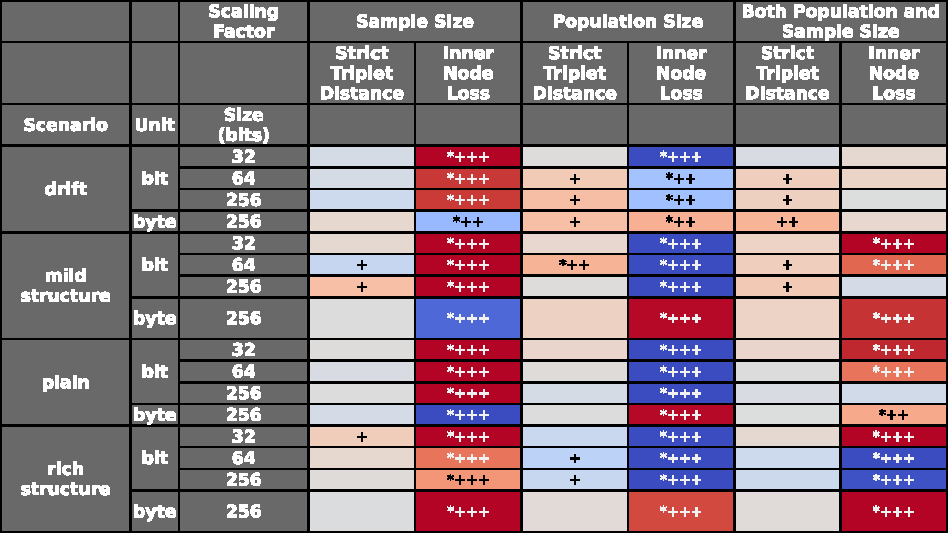
\includegraphics[width=\textwidth]{binder/binder/dsamp-popsize-scale/outplots/dsamp-popsize-scale-tilted.pdf}
  \caption{%
   \textbf{Comparison of reconstruction quality between small and large downsample and population sizes under tilted retention policy.}
   \footnotesize
    First column considers sample size in isolation, second column considers scaling population size in isolation, and third column considers scaling population and sample size together.
    Color coding reflects non-parametric comparison between quality measure values, with red indicating degraded reconstruction quality at larger scale and blue indicating improved reconstruction quality at larger scale.
    Bigger downsample size is 8,000 taxa and smaller downsample size is 500 taxa.
    Bigger population size is 65,536 and smaller population size is 4,096.
    Experiments used tilted retention policy with surface-based implementation.
    In cell annotations, +'s indicate small, medium, and large effect sizes using the Cliff's delta statistic and *'s indicate statistical significance at $\alpha = 0.05$ via Mann-Whitney U test.
  }
  \label{fig:dsamp-popsize-scale-tilted}
\end{figure*}
